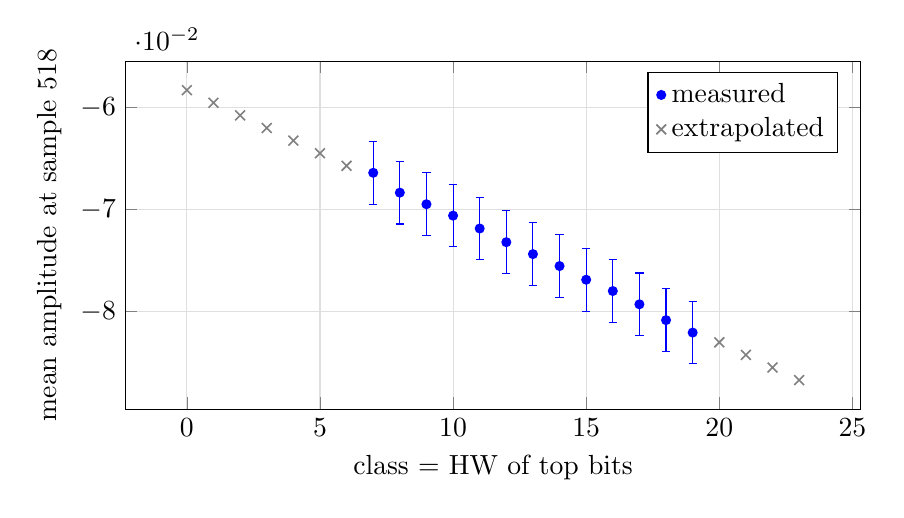
\begin{tikzpicture}
\begin{axis}[
  xlabel={class = HW of top bits},
  ylabel={mean amplitude at sample 518},
  width=0.9\linewidth,
  height=6cm,
  grid=major,
  grid style={gray!25},
  legend pos=north east,
  legend cell align=left,
]
\addplot[blue, semithick, mark=*, mark size=1.5pt, only marks, error bars/.cd, y dir=both, y explicit, error bar style={blue}] coordinates {(7,-0.0664062) +- (0,0.00306939) (8,-0.0683511) +- (0,0.00306939) (9,-0.069486) +- (0,0.00306939) (10,-0.0706037) +- (0,0.00306939) (11,-0.0718664) +- (0,0.00306939) (12,-0.0732073) +- (0,0.00306939) (13,-0.0743762) +- (0,0.00306939) (14,-0.0755463) +- (0,0.00306939) (15,-0.0768886) +- (0,0.00306939) (16,-0.0779954) +- (0,0.00306939) (17,-0.0792961) +- (0,0.00306939) (18,-0.0808478) +- (0,0.00306939) (19,-0.0820677) +- (0,0.00306939)};
\addlegendentry{measured}
\addplot[gray, semithick, mark=x, mark size=2.5pt, only marks] coordinates {(0,-0.058308) (1,-0.0595435) (2,-0.0607791) (3,-0.0620147) (4,-0.0632502) (5,-0.0644858) (6,-0.0657214) (20,-0.0830193) (21,-0.0842549) (22,-0.0854904) (23,-0.086726)};
\addlegendentry{extrapolated}
\end{axis}
\end{tikzpicture}
